\documentclass[letterpaper,twocolumn,10pt]{article}
\usepackage{usenix2019_v3}

% to be able to draw some self-contained figs
\usepackage{tikz}
\usepackage{amsmath}
\usepackage{graphicx}

\graphicspath{ {./images/} }

%-------------------------------------------------------------------------------
\begin{document}
%-------------------------------------------------------------------------------

%don't want date printed
\date{}

% make title bold and 14 pt font (Latex default is non-bold, 16 pt)
\title{\Large \bf Density Based Clustering for Hierarchical and Autonomous Fog Architecture}

%for single author (just remove % characters)
\author{
{\rm Robin C.\ Ward}\\
PhD Student\\
Auburn University\\
Auburn, Alabama 36849\\
Email: rcw0024@auburn.edu\\
} % end author

\maketitle

%-------------------------------------------------------------------------------
\begin{abstract}
%-------------------------------------------------------------------------------
When given a finite resource such as the space on planet Earth, and add a rapidly growing population (there is approximately a net gain of one new person on the planet Earth every 31 seconds\footnote{\url{https://www.census.gov/popclock}}), there will become a growing need to group the growing number of devices in a much faster method. This is where adding the DBSCAN method into HAFA~\cite{10.1145/3229710.3229740} would greatly reduce the overall average case run time. 


Figure~\ref{fig:backup} for the location of the new button.

\begin{verbatim}
put psuedocode here
\end{verbatim}

\end{abstract}


%-------------------------------------------------------------------------------
\section{Introduction}
%-------------------------------------------------------------------------------

In the following sections, many areas will be covered such as the new features added to the VCG tool, the importance of them, some of the code%
\footnote{VCG uses Visual Basic .NET} that was required to implement them as well as future improvements. In addition to explaining the new additions that were added to the VCG tool, each following section will include a subsection that will also contain possible improvements and/or advancements that could be added on top of what has already been done. These additions, though may seem small, should prove to be a worthy addition to the VCG tool. It is also recommended that the reader download%
\footnote{\url{https://sourceforge.net/projects/visualcodegrepp}} and install the VCG tool and become familiar with all of its features. A list of other similar tools as well as the VCG tool can be found See 

\subsection{Possible Improvements}
\begin{description}
\item[configuration file select] One possible improvement that would make the backup feature better would be the addition of a multi-select backup. This would allow the user to select which configuration files they would like to backup. 
\item[progress bar] Another improvement which may prove to be useful would be the addition of a progress bar when backing up the local files. Even though the process is very fast, sometimes a visual indicator is still nice to have, especially if the files grow in size as time goes on.
\end{description}

\begin{figure}[h]
\centering
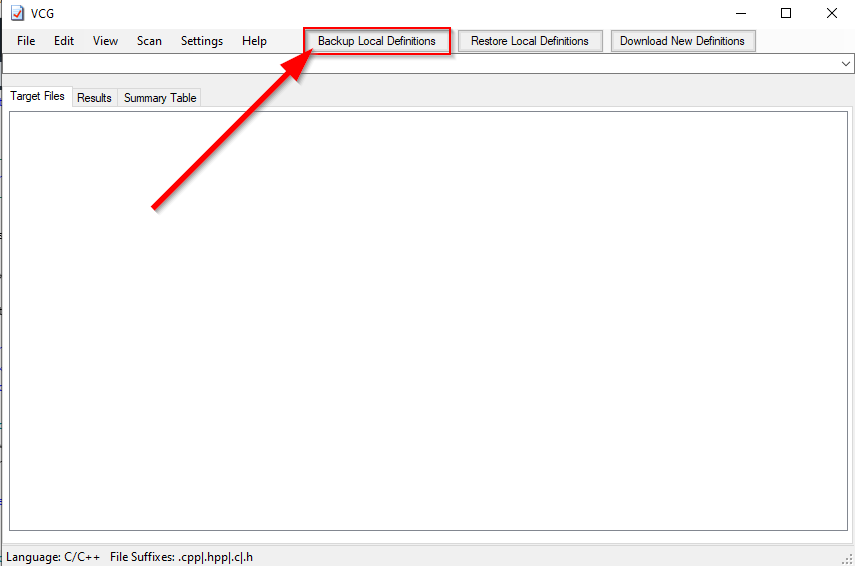
\includegraphics[width=0.45\textwidth]{backup}
\caption{\label{fig:backup}Location of the new "Backup Definitions" button.}
\end{figure}

\bibliographystyle{plain}

\bibliography{bibliography.bib}
%%%%%%%%%%%%%%%%%%%%%%%%%%%%%%%%%%%%%%%%%%%%%%%%%%%%%%%%%%%%%%%%%%%%%%%%%%%%%%%%
\end{document}
%%%%%%%%%%%%%%%%%%%%%%%%%%%%%%%%%%%%%%%%%%%%%%%%%%%%%%%%%%%%%%%%%%%%%%%%%%%%%%%%

%%  LocalWords:  endnotes includegraphics fread ptr nobj noindent
%%  LocalWords:  pdflatex acks